%%
%% Copyright 2007, 2008, 2009 Elsevier Ltd
%%
%% This file is part of the 'Elsarticle Bundle'.
%% ---------------------------------------------
%%
%% It may be distributed under the conditions of the LaTeX Project Public
%% License, either version 1.2 of this license or (at your option) any
%% later version.  The latest version of this license is in
%%    http://www.latex-project.org/lppl.txt
%% and version 1.2 or later is part of all distributions of LaTeX
%% version 1999/12/01 or later.
%%
%% The list of all files belonging to the 'Elsarticle Bundle' is
%% given in the file `manifest.txt'.
%%

%% Template article for Elsevier's document class `elsarticle'
%% with harvard style bibliographic references
%% SP 2008/03/01
%%
%%
%%
%% $Id: elsarticle-template-harv.tex 4 2009-10-24 08:22:58Z rishi $
%%
%%


%% WHAT WE WERE USING \documentclass[final,authoryear,11pt,times]{elsarticle}

%% Use the option review to obtain double line spacing
%% \documentclass[authoryear,preprint,review,12pt]{elsarticle}

%% Use the options 1p,twocolumn; 3p; 3p,twocolumn; 5p; or 5p,twocolumn
%% for a journal layout:
%% \documentclass[final,authoryear,1p,times]{elsarticle}
%%\documentclass[final,authoryear,1p,times,twocolumn]{elsarticle}
%%\documentclass[final,authoryear,3p,times]{elsarticle}
%%\documentclass[final,authoryear,3p,times,twocolumn]{elsarticle}
\documentclass[final,authoryear,5p,times,twocolumn]{elsarticle}

%% if you use PostScript figures in your article
%% use the graphics package for simple commands
%% \usepackage{graphics}
%% or use the graphicx package for more complicated commands
%% \usepackage{graphicx}
%% or use the epsfig package if you prefer to use the old commands
%% \usepackage{epsfig}

%% The amssymb package provides various useful mathematical symbols
\usepackage{amssymb}
\usepackage{amsmath}

%%\usepackage[margin=1.25in]{geometry}


\usepackage{todonotes}
\usepackage{epigraph}
\usepackage{graphicx}
\usepackage{setspace}
\usepackage{hyperref}
\renewcommand{\sectionautorefname}{\S}
\renewcommand{\subsectionautorefname}{\S}
\onehalfspacing

%% The amsthm package provides extended theorem environments
%% \usepackage{amsthm}

%% The lineno packages adds line numbers. Start line numbering with
%% \begin{linenumbers}, end it with \end{linenumbers}. Or switch it on
%% for the whole article with \linenumbers after \end{frontmatter}.
%% \usepackage{lineno}

%% natbib.sty is loaded by default. However, natbib options can be
%% provided with \biboptions{...} command. Following options are
%% valid:

%%   round  -  round parentheses are used (default)
%%   square -  square brackets are used   [option]
%%   curly  -  curly braces are used      {option}
%%   angle  -  angle brackets are used    <option>
%%   semicolon  -  multiple citations separated by semi-colon (default)
%%   colon  - same as semicolon, an earlier confusion
%%   comma  -  separated by comma
%%   authoryear - selects author-year citations (default)
%%   numbers-  selects numerical citations
%%   super  -  numerical citations as superscripts
%%   sort   -  sorts multiple citations according to order in ref. list
%%   sort&compress   -  like sort, but also compresses numerical citations
%%   compress - compresses without sorting
%%   longnamesfirst  -  makes first citation full author list
%%
%% \biboptions{longnamesfirst,comma}

% \biboptions{}

\journal{CS280r, Spring 2017 - Final Project Report, Goldstein and Wihl}

\begin{document}

\begin{frontmatter}

%% Title, authors and addresses

%% use the tnoteref command within \title for footnotes;
%% use the tnotetext command for the associated footnote;
%% use the fnref command within \author or \address for footnotes;
%% use the fntext command for the associated footnote;
%% use the corref command within \author for corresponding author footnotes;
%% use the cortext command for the associated footnote;
%% use the ead command for the email address,
%% and the form \ead[url] for the home page:
%%
%% \title{Title\tnoteref{label1}}
%% \tnotetext[label1]{}
%% \author{Name\corref{cor1}\fnref{label2}}
%% \ead{email address}
%% \ead[url]{home page}
%% \fntext[label2]{}
%% \cortext[cor1]{}
%% \address{Address\fnref{label3}}
%% \fntext[label3]{}

\title{$A \rho \mu o \nu \acute{\iota} \alpha$ (Harmonia): A System for Collaborative Music Composition}

%% use optional labels to link authors explicitly to addresses:
%% \author[label1,label2]{<author name>}
%% \address[label1]{<address>}
%% \address[label2]{<address>}

\author{{\rm Mark Goldstein, David Wihl}\\ Harvard University}
\address{\normalsize\{markgoldstein,davidwihl\}@g.harvard.edu}

\begin{abstract}

Increasing productivity of music composition has many positive benefits. Listeners would appreciate individually tailored music to their emotional needs and context. Composers would be facilitated by greater and more diverse cooperation yielding more innovative music. Composition agents could assist in the generation of repetitive or  experimental musical forms. Therapists can use music as part of a treatment plan  for autism and many other disorders. The system we propose attempts to address these myriad needs  by offering two key innovations: a SharedPlan with collaborative versioning to mediate the workflow of a composition for a group of musicians, an algorithmic evaluation of a composition against the intention of the SharedPlan to provide guidance to both human and agent composers.

\end{abstract}

\end{frontmatter}

%\title{\Large $A \rho \mu o \nu \acute{\iota} \alpha$ (Harmonia): A System for Collaborative Music Composition}
%\author{{\rm Mark Goldstein, David Wihl}\\Harvard University}
%\address{\normalsize\{markgoldstein,davidwihl\}@g.harvard.edu}
%\maketitle


%\section{Abstract}
%\label{sec:abstract}

%Increasing productivity of music composition has many positive benefits. Listeners would appreciate individually tailored music to their emotional needs and context. Composers would be facilitated by greater and more diverse cooperation yielding more innovative music. Composition agents could assist in the generation of repetitive or  experimental musical forms. Therapists can use music as part of a treatment plan  for autism and many other disorders. The system we propose attempts to address these myriad needs  by offering two key innovations: a SharedPlan with collaborative versioning to mediate the workflow of a composition for a group of musicians, an algorithmic evaluation of a composition against the intention of the SharedPlan to provide guidance to both human and agent composers.

\section{Introduction}
\label{sec:introduction}

\epigraph{It is my design to render it manifest that no one point in its composition is referrible either to accident or intuition -- that the work proceeded, step by step, to its completion with the precision and rigid consequence of a mathematical problem.}{\textit{Edgar Allen Poe, The Philosophy of Composition}}

\todo[inline]{Mark: Need to reword this first paragraph}

Music composition is often an individual endeavor, which is counterintuitive when music is mostly performed, improvised, and experienced in a group. Part of this is due to the singular nature of creative expression, but a large part is also due to a dearth of viable tools to enable collaborative efforts between composers. Most modern composition is facilitated through the use of digital workstation tools, yet composers do not generally have access to tools designed for collaboration, version control, and annotation that are available to software engineering teams.

There are many additional issues that surround collaboration over structured, shared objects such as a music composition. Each composer has a strong artistic vision, and a composer working on one section of a piece may ruin the plans of another working on a later section. It is crucial in such settings that a group specify an artistic goal and communicate their intentions for material as it is added. However, a valuable aspect of art in such settings is that new ideas can surface specifically because of the give-and-take of the collaborative process, leading to material that could not be created by any one artist. How can composers stay connected with an original goal and also make room for spontaneity as a result of the collaborative setting?

Collaborative Ideation (CI) investigates the effect of various idea-sharing tactics on the creativity, productivity and scope of individual idea-generating participants. Such techniques may include showing each participant in a pool of brainstormers the collection of all participants' brainstormed ideas. In CI that focuses on the creation of shared (as opposed to individual) objects or solutions such as a composition or story, it may be the case that certain interfaces for collaboration, certain automated, filtering idea-sharing mechanisms for collaborators, and certain per-participant feedback from the system may help facilitate group creativity and productivity toward a shared goal.

SharedPlans provide a framework to establish and maintain context and metadata about group artistic work. This framework ensures that the collaborative process and ideation stay within reasonably agreed parameters, provides a formalized notion of common beliefs and defines a mean of independent instrumentation that the work-in-progress is navigating toward the original intention.

We propose a system that addresses collaborative music composition inspired by tools used for software teamwork, collaborative ideation, and musical structure analysis. This system defines an interface for collaboration over a shared creative artifact, and includes procedures for editing a work-in-progress and receiving algorithmic  feedback about edits. Crucially, the system assists collaborators with the task of staying on track with an \textit{a priori} specified goal for the turnout of the piece, and also provides a framework for communication among collaborators about the intention of edits during collaboration.

We first examine previous work related to shared intentionality, collaboration and group ideation, intelligent music systems, and modeling the structure of music. Next, we describe the details of the overall usage workflow, as well as the individual components of our system. This includes a specification of an automated approach for giving composers feedback on the relevance of their ideas to a specified collaborative goal. We present three use cases for our system, where collaborating composers create music ranging in purpose from casual listening to clinical therapy. We conclude with a discussion of our system proposal, including limitations we have identified and potential future work.

%Deep Neural Networks are being used for the creation of new visual[ref to Sketch paper], narrative[ref] and now musical works[wavenet? magenta ref?]. These sophisticated tools can assist a human composer with idea exploration and generation, as well as with idea evaluation (e.g. a composer may evaluate the likelihood of a musical sample against a corpus).

% parts of system may be replaced by DNNs

\section{Related Work}

%TODO Discussion of previous important, similar work in the area with comparison to the particular approach taken and results of the paper. Avoid simply providing a laundry list of other work that is somehow related to the subject of the paper. This section should contain brief, in depth discussions of the work most similar to your project, i.e., to research that takes an approach to the problem or produces results with which your project should be compared. As is always the case with written work, throughout the paper you should have citations to work that you draw on. For example, if you have adapted a system, include a citation to the system when you first mention it; if you are extending a formalization, include a citation to the original on first mention. If you are unclear about whether a simple citation suffices or an extended discussion is needed in the Related Work section, look at the papers read for class this semester for models. If you are still unsure, check with the teaching staff.

Our work builds on several areas of research related to music, computer science, and creative cognition. First we discuss related work regarding shared intentionality in multi-agent settings. Then we discuss collaborative ideation, both in general and specifically in music. Next we discuss intelligent music systems that facilitate human composition and improvisation, and related work in Music Information Retrieval (MIR). Finally we describe previous work that applies information theory to the analysis of musical structure.

\subsection{Shared Plans}

SharedPlans [Grosz, Hunsberger] define a robust framework for multiagent, multi-level collaboration. A SharedPlan consists of a set of intentions, mutual beliefs, constraints, and hierarchies of actions and plans. All of these elements are applicable in this context, although only a subset of the general definition is needed for music composition purposes. 

A SharedPlan is the basic unit of work. It serves as the container for the initial definition of the intent of the work, the musical score representing the work-in-progress, the revision history of the work-in-progress, the sub-plans used to communicate between composers, and the final approval given by the user(s) who defined the SharedPlan initially.

Intentions are expressed by a minimum of two criteria: genre and mood. Genre and mood are algorithmically combined using existing methods [TODO: specify forward reference] to define the approximate representation of the final work.
  
Mutual beliefs are expressed in the trust of the algorithmic evaluation of genre / mood combination as well as the algorithmic evaluation of the musical structure. This extends the notion of beliefs in SharedPlans to a predictable instrumentation of common understanding, simplifying integration of both human and agent composers. 

There is but one complex action and one Full SharedPlan in this scenario: production of a score that meets the intention. Each composer may divide the complex action into a series of sub-actions [See section xxx]. If a composer is unable to complete all actions necessary to achieve the intention, a sub-plan is created stating the Intention-To for a future composer. This is primary means that composers communicate with each other. We do not define a means of using \textit{recipes} in this context.

We use the term composer in the singular form, however a single composer may consist of several collaborating humans to produce a single action on the score. Any such informal communication or experimentation is beyond the scope of our proposal. After collaborating, a single human would execute an action or set of actions to advance the composition towards the intented goal. For example, a human composer may improvise with colleagues to explore several alternatives of a sub-plan. Once a consensus is achieved that the section meets artistic and SharedPlan goals, the one composer performs one action on the SharedPlan. 


\subsection{Collaborative Ideation}
% Collaborative Ideation In General
Collaborative Ideation (CI) seeks to improve the productivity of individuals and groups in generating ideas through collaboration. The people involved are interested in creating related objects (e.g., we all want to brainstorm solutions to social problems) and seek either feedback or examples of others' work to enhance their individual process. Collaboration is centered around a shared workspace, physical or virtual, that allows for communication and sharing of ideas. The ideas produced may be for individual use, or ideators may work on shared artifacts such as an essay or piece of art. The dynamics of collaboration may be real-time or not, though increasingly, today's settings are real-time and virtual [TODO: find citation]. A simple CI setting is one where each ideator brainstorms solutions to a problem common to all participants, and each participant can see all other's ideas. While such approaches have been used naturally in human culture for millennia, the design of intelligent computer systems today aims to facilitate these activities to allow for increased creativity and productivity. 

%IdeaHound
It has been shown that only a small subset of an idea pool may be relevant and inspiring to a single ideator, and that it is overwhelming for each ideator to view all participant's ideas [Siangliulue's 2015]. In IdeaHound [Siangliulue 2016], each user is prompted to interact with a personal ``whiteboard`` where they can cluster their ideas and separate them by semantic distance as they generate them. The system then creates a global semantic map of all generated ideas from the whiteboards, which allows each ideator to easily view their work in the context of the entire solution space. Using this map, IdeaHound recommends diverse suggestions to each ideator, eliminating the cognitive load of idea search. In the collaborative composition setting, CI is implicitly present in the individual work of each composer. By working on material of multiple stylistic origins, composers may come up with things they would make on their own. CI is made explicit when a composer addresses a SharedPlan sub-goal instantiated by another [See section XXX]. In our work, generated objects are structured, rather than unordered collections of ideas, and ideators need to build over each other's ideas rather than only seek inspiration from examples by others. These details present new challenges.


%Soundcloud and Blend
CI has surfaced in a setting closer to ours, in the space of online blogs and services designed to share visual art and music. Ideas range from small, unfinished efforts seeking direction to finished pieces seeking critique. Artists improve upon their ideas using large-scale feedback. SoundCloud is a hybrid music streaming service and CI platform. Though music is often presented in finished form, people also post incomplete projects. Artists sometimes share ``stems" to their music, which are individual sound files that feature isolated instrumental tracks, with the intention that others seeking inspiration remix their pieces into new work. The Blend platform \footnote{\texttt{https://blend.io}} makes the sharing of source files explicit. By default, artists share their works-in-progress in the format of music production software source files, which allows others to quickly pick up on their work. This setting encourages building on each other's ideas. However, people mostly build on other's work toward an ultimately individual direction. What changes when several ideators intend to create a shared piece? In our work, a composition may have a collaboratively-specified goal associated with it through the duration of its existence. It is up to the composers and the system to keep a piece of music close to its SharedPlan.

\subsection{Computer Facilitated Composition and Improvisation}

% Music Info Retrieval in General
Intelligent Music Systems ranging from composition and improvisation facilitiating agents to recommendation systems have a common requirement, to ``understand" music at multiple levels, including low-level acoustic signal, mid-level theoretical constructs such as harmony and rhythm, and high-level level aspects such as mood, genre, and style. For example, a music recommendation system such as Spotify \footnote{\texttt{https://www.spotify.com}} seek to analyze music and extract a measure of relevance for a function such as "study music". These issues constitute the research area of Music Information Retrieval (MIR).

% ChordRipple
In systems that create music, the interest is to assist human composers, rather than replace them. Perhaps a composer has good ``seeds" ideas, but the system may recommend variations of ideas, or re-orderings of ideas, to make them more conveying. Such system knowledge often comes from large-scale corpus analysis that mines patterns common to a collection of music. ChordRipple [Huang 2016] takes as input a progression of musical chords from a composer, and suggests substitutions of intermediate chords that preserve the original semantics of the input while serving to replace conventional choices with more interesting ones. If the composer agrees to make one of the recommended changes, the system assists the composer in interpolating between original and substituted material before and after the initial substitution, resulting in further mixing of human and system generated music. Our system makes suggestions to composers, but it focuses on structural changes rather than material substitutions to support collaboration.

% Magenta and AI Duet
While our current work seeks primarily to assist teams of human composers to enrich and organize their work, we intend to design the system such that intelligent computer agent composers may fully participate without requiring human intervention. Last year, Google Brian launched the Magenta Project for exploring machine intelligence in music \footnote{\texttt{https://magenta.tensorflow.org/welcome-to-magenta}}. Magenta is an integrated environment of software tools and music-related datasets. This year, Magenta released AI Duet \footnote{\texttt{https://aiexperiments.withgoogle.com/ai-duet}}, a computer system that reacts to human improvised gestures. Improvisation is an important part of composition. When a single composer is brainstorming, it may be beneficial to improvise on ideas with an automated agent, much like two musicians iteratively vary and refine their ideas in live rehearsals. In settings where a piece is defined by a specific enough set of guidelines [See Therapy use case in Section XXX]  where a listener may need music at a certain tempo and with a simple beat, powerful information retrieval systems may make effective machine composition agents possible. Human composers may be placed at later steps of collaboration to ensure that the piece meets requirements in humanly perceptible ways.

\subsection{Information Theory and Music Analysis}

Our systems relies on the ability to model musical structure in a way that supports automated feedback for collaborating composers, where feedback is in the form of suggested rearrangements of musical ideas that help a composition reach a mutually specified structural goal. In this direction, there has been a rich body of work in automated analysis of musical structure from the 1950's to present. A prominent direction is to model musical form by way of listener perception and the expected dynamics of their attention and surprise. Understanding musical structure and its impact on listeners is a cogent goal to music theorists, cognitive scientists, and machine learning researchers. Many of these approaches have drawn on probability theory and information theory. A survey of approaches historical to contemporary can be found in the Con Espressione Manifesto [Widmer 2016], which is a strong position paper on the coming decade of research directions for music information retrieval. Many of these works borrow from original principles described in \cite{shannon} in largely unmodified ways.

% Abdallah, Predictive Information Rate
Our work builds on the Information Dynamics Approach [Abdallah et al 2012]. Abdallah uses predictive information rate, a entropy/divergence based metric that measures how a listener's mid-piece distribution over future musical events is continually revised as new information is presented, to compute a curve that summarizes aspects of surprise in redundancy in a piece of music. Our work assumes that musical structure can be effectively summarized by this criteria. We assume that pieces from a particular genre/mood are defined by characteristic balances of surprise and redundancy over time, with peaks of information content (communicated by the composer) in genre-specific locations. We leverage this metric as the foundation of our automatic analysis system, which compares a collaborative work-in-progress against the characteristic curves for the genre and mood specified by the work's SharedPlan, and suggests edits to the composers to keep them in line with their goal.

\section{System Design}

After reviewing the typical workflow of a editing a piece of music as part of a team of composers, we describe the details of our system design. The design is centered around addressing two aspects of collaborative composition. The first includes the composition interface, the representation of music, the editing capabilities of composers, and the version control system used to track musical revisions. These all focus on issues of communication and coordination in collaboration over a shared artifact of a specified format, and with a specification of editing actions. Then we discuss the automated music analysis used in our system for giving feedback and suggestions to composers. This facilitates the collaborative composition process by helping composers assess the affect of their edits on the movement of the work in progress toward the goal, and is specific to the domain of music. We discuss how these two system functions in combination help composers by guiding aspects of revision on a shared musical artifact, and by providing an interface that makes such revisions convenient, modular, and amenable to collaboration.

\subsection{Workflow Overview}

\begin{figure}
	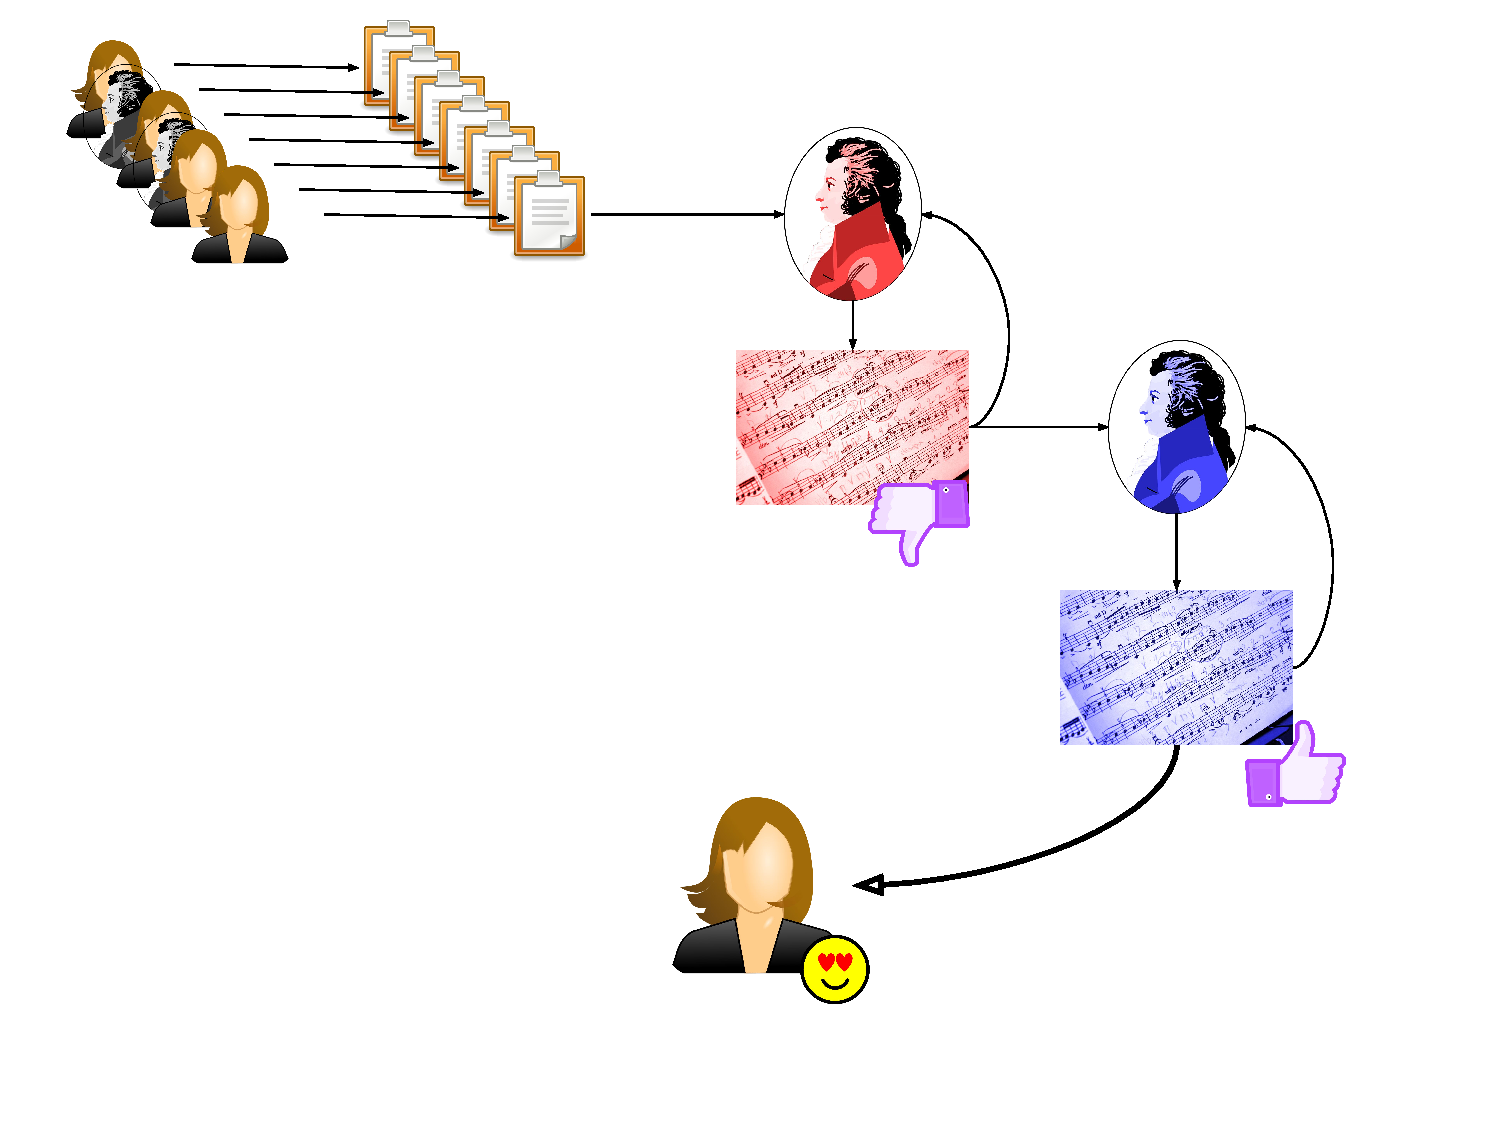
\includegraphics[scale=0.35]{workflow.pdf}
	\caption{Overall workflow: a non-musical user or a composer define a SharedPlan. Composer 1 (\textcolor{red}{red}) starts
	iterating and commits a work-in-progress. Composer 2 (\textcolor{blue}{blue}) continues iterating until the original user is
	satisified.}
	\label{fig:workflow}
\end{figure}

The generic use case that we consider is that a listener (musician or not) requests a new piece of music of a specified genre and mood, and perhaps other related keywords. A new, blank score is associated with a metadata file that stores the information about the goal keywords, and additional information later. An information retrieval system uses as much of the metadata keywords as it can to retrieves MIDI scores for existing related works. The system then computes a summary of characteristic musical structure of the retrieved body of work.

As composers begin to work on the piece, they iterate adding and editing material, and receiving feedback from the system about their edits. The system computes the similarity of the structure of the composition-in-progress to the characteristic intent structure, and helps composers choose which edits are most relevant. The system also suggests edits that align with bringing the composition closer to the goal, for example switching the order of two parts of the composition. Composer can follow suggestions or do their own modifications, or do nothing and finish an iteration. During this process, composers commit additional metadata describing the intentions of local edits, such that others can pick up on their material and preserve these intentions. The composers collaborate to bring the composition to a state of completion such that it matches the originally specified goals. Composers iterate on the composition until the music requester(s) is/are satisfied. The finished product is a MIDI score for a piece of music.
 


\subsection{Version Control}

Version control has become an essential part of team-based software development. However, the tools for managing
revisions of other creative work, including music composition, are non-existant or limited in comparison. There are
two commercial version control systems for music: the aforementioned Blend and Splice.com \footnote{\texttt{https://splice.com/}}. \texttt{git} [Torvalds] has been referenced elsewhere [Wolf] as a viable means for musical score version control, especially in the MIDI format.

Software based version control systems are excellent for basic version control operations such as branching, committing and viewing history, there are lacking several primitive necessary for integration in our proposed workflow. In the interest of brevity, we do not specify the entire subset of major \texttt{git} commands necessary for version control.

In addition to \texttt{git}'s extensive functionality, we propose the following additional commands for the workflow:

\noindent For users and composers:
\begin{description}
    \item [EditPlan] - create, revise or delete a SharedPlan that includes intentionality and other metadata.
    \item [Approve] - the SharedPlan creator denotes a SharedPlan as satisfactorily executed
    \item [Reject] - the SharedPlan creator denotes a SharedPlan as unsatisfactorily executed
\end{description}

\noindent For composers only:
\begin{description}
    \item [Evaluate] - prior to committing a revision, perform an analysis of the current score against intentionality.
    \item [EditSubplan] - create, revise or delete a sub-plan. Creating or editing a sub-plan would establish the hierarchical context to the SharedPlan.
    \item [Release] - after a commit, mark a plan or sub-plan as ready for review by the creator of the SharedPlan. This implicitly closes the sub-plan.
\end{description}

The versioning aspect is particularly relevant in the music context, as intellectual property and originality is often the source of extensive lawsuits. By maintaining version control, an examination of the history would assist in the identification of derivative works and originality of authorship.

\subsection{Sub-plan as Inter-composer Communication}
 
When a composition task is created, it exists as a SharedPlan that contains an intent specification, as well as a \texttt{NULL} score. The initial specification must meet a minimal criteria, which is that a genre and a mood must be specified. However, additional descriptive keywords may be included, of the style that typically comes in the form of tags on YouTube or Soundcloud ($\#$USA, $\#$lo-fi, $\#$chill, $\#$electronic, $\#120BPM$). These tags power an automated comparison between work-in-progress and goal, and helps composers pick edits that may bring a composition closer to a sound characterized by the goal keywords. In particular, we assume that an information retrieval system for querying large amounts of music by keyword exists, and retrieves MIDI scores to be analyzed by our system.

In addition to containing initial goal-describing information, the sub-plan is responsible for mediating any inter-composer communication that takes place aside from the edits to the shared musical work itself. The sub-plan may be updated actively as the piece is revised. A composer may wish to express the intention of a particular edit to justify its presence or to elicit specific future directions for their material. For example, a composer may add a block of music containing an exposed melody, but may want to communicate that another composer should add a harmonic accompaniment to that section.

It is ideal for such communication to be concise and structured. It may be detrimental to collaborative work for one participant to expect all other participants to read five paragraphs of unstructured goal descriptions for a particular section of music. Such a message may require too high of a cognitive load for the others to carefully read and understand, and the intending composer may not have their ideas respected. We have not yet designed a structured language for including block-specific comments enabling composers to share local intents per-edit, but our system allows small free-form comments to be included. A structured language may help support automated agent collaborators in the future. This is discussed further in the Therapy case study (See section BLAH). Providing a mechanism for composers to share there intentions per-edit is crucial because it can help to distinguish between two kinds of composer misunderstandings/disagreements. The first scenario is where a composer agrees with another composer's intention about an edit, but disagrees with the actual implementation. This may lead to the second composer editing the first composer's material with care to preserve the original sound, or replacing it with something of similar affect. The second scenario is where a composer fundamentally disagrees with the artistic intention of another. An effective SharedPlan communication system may disambiguate these cases.

\begin{figure}
\vspace*{-3cm}
	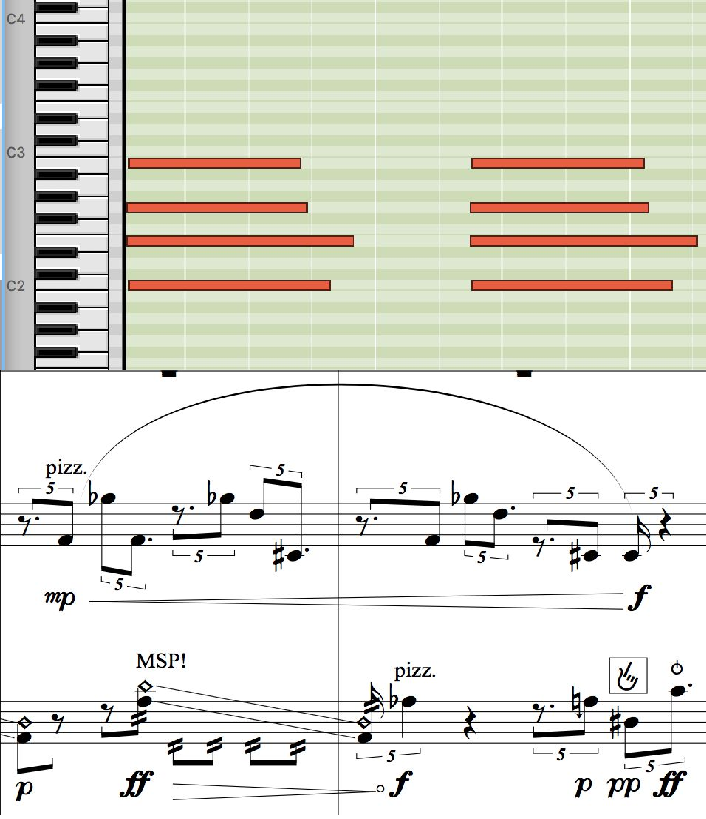
\includegraphics[scale=0.4]{midi.pdf}
	\caption{MUST FIX THIS IMAGE SPACING. Top: MIDI. Bottom: MusicXML}
	\label{fig:midi}
\end{figure}

\subsection{MIDI and Edit Actions}

Our system represents music in MIDI format. MIDI is a protocol for communicating discrete information about the pitch, duration, and dynamics of individual notes. A musical work is described by specifying the vertical arrangement of individual notes as chords and their horizontal arrangement over time. Additionally, there is a General MIDI Soundbank that maps integers to specific electronic instrument sounds. For example, one can specify that this MIDI part is meant to be played by sound $0$, grand piano or Ocarina, sound $80$. Most familiar software for music notation and music production build user interfaces on top of a basic MIDI file editor. Extensions to this protocol include MusicXML, which allows for the specification of additional parameters such as expression markings and articulation information. In this initial specification, a simple MIDI editor is sufficient. Through the use of additional metadata (next section), composers are able to segment MIDI files into separate segments. For example, a piece may be subdivided into several sections. Segmentation may represent intentions about musical form, for example one may segment part of a composition into an exposition and a development section. 
\todo[inline]{David: $\uparrow$ I suggest moving MusicXML to Future Work to avoid clutter here.}

During an interaction with the system, a composer is able to change a composition by editing the MIDI in several low-level or high-level ways. Composers can add a new block of material, edit an existing block, remove an existing block, swap the order of two blocks, merge two blocks, or split a block into two. At each iteration of editing, the system suggests an option that may bring the work in progress closer to what is specified by the SharedPlan. This is primarily of the form of "switch blocks A and B?" (See Section on Automatic Evaluation). The final product of collaboration is a MIDI file that represents the pitches, rhythms, and dynamics of musical events, as well as a collection of metadata that concisely states additional information, such as tempo and instrumentation. 

\begin{table}
    \begin{tabular}{|l|l|}
    	\hline
    	\textbf{Action} & \textbf{Description} \\
    	\hline
    	\textit{Insert,Delete,Replace} & Add, remove or replace a block \\
    	\textit{Move} & Rearrange order of a block \\
    	\textit{Split, Merge} & Divide or combine a block \\
    	\hline
    \end{tabular}
	\caption{Summary of Atomic Edit Actions on Score}
\end{table}

The piece can be produced as an electronic piece of music by importing the MIDI into any music production software, specifying which MIDI track should be played by which sound or synthetic instrument, and exporting a sound file. If desired, composers may take additional actions on that finished work that are external to the system, such as produce the piece of music with live musicians or extended software instruments, but this is beyond our scope, which is mainly to facilitate collaboration during the composition process.

\subsection{Design Failure Modes}

There are multiple potential failure circumstances of the proposed design:

\begin{description}
\item[Failure to compose] No composer may elect to work on a given SharedPlan.
\item[Failure to satisfy] The creator of the original SharedPlan may never approve or reject the produced work, leaving it in an undefined state.
\item[Sub-plan not released]A sub-plan may be defined but no composer ever completes the sub-plan so the work stays in an incomplete state.
\item[Evaluation not converging] The evaluation process may continue to offer suggestions that are rejected by the composer. Note that the evaluation process only makes recommendations but is not a gatekeeper for the composer to release. However, if the Evaluation mechanism repeatedly gives undesired or unhelpful suggestions, composers will cease future use.
\item[Fail to Evaluate] there may not be sufficient training data for a given genre / mood combination so the Evaluation may fail to provide sufficiently useful recommendations.
\end{description}

None of these failure modes results in a castastrophic collapse of the system. Failures result in a specific SharedPlan not advancing but does not preclude other SharedPlans from continuing to evolve.

\section{User Interface}

There are three aspects to the user interface: for non-musical users, for composers performing workflow and for composers actively editing the musical score.

\subsection{SharedPlan Workflow User Interface}

There are four commands possible in this context: \textbf{EditPlan} (including create/edit/delete), \textbf{Approve, Reject}. Since the user may not have any musical background, this user interface should be accessible to as large a population as possible. Ideally, this would be a simple looking, reactive web-based interface that would work equally well on mobile devices as well as desktops. Music apps such as Spotify may wish to integrate this functionality so a web-based API should also be accessible.

For an unsophisticated user, \textbf{Approve} and \textbf{Reject} may be considered implicit. If the user listens to the composition past a certain point, such as 80\% of the total length of the work, it may be deemed implicitly approved. Similarly, if the user advances to another song within the first 20\%, the composition is implicitly rejected. Implicit rejection does not provide any causal reason for the rejection, so trial and error analogous to reinforcement learning must be used to discover the hidden reasons why a work was implicitly rejected. Other user actions (such as stopping all music in the middle of play) do not provide enough signal to determine implicit actions so the work's acceptance status remains unknown.

\subsection{Sub-plan Workflow User Interface}

The market reality is the most modern composers use an existing Digital Audio Workstation (DAW) such as Ableton or LogicPro. Rather than replacing the composer's primary user interface, integration should be performed within the menu system of the most common DAWs. There are only two commands required in this context: \textbf{EditSubplan} (including create/edit/delete) and \textbf{Release}. 

%  how do composers view metadata? How specifically do they view metadata associated with a particular block. Maybe when they click a block, any existing metadata about it opened. So if I click a block with a melody, I may see that the melody composer asked to add a chord under the melody. Do these notes go away? Can the second editor close the request? Does the original poster need to approve? Maybe the second editor can close it, and the original editor can add a new note later if they are still not happy?  David's response: I think the Release command effectively closes the sub-plan. Anyone working on the SharedPlan can create or release a sub-plan.


\subsection{Composer Edit / Evaluation User Interface}

This is most complex and demanding user interface as it requires the highest degree of interactivity. Rather re-implementing the multitude of music editing features of a mature DAW, integration to existing DAWs is again preferable over creating a \textit{de novo} user interface. 

The most novel aspect would be the integration of the evaluation to the editing task. Ideally the evaluation result would decorate and annotate the score enabling the composer to address results of the evaluation while remaining in a known editing context, analogous to seeing and resolving comments in Microsoft Word or a Google Doc.

 
 

\section{Automated Analysis of Musical Structure}

Harmonia facilitates collaborative composition in two ways. First, the interface as a whole, including the revision system an the shared metadata associated with each composition, helps with practical aspects of communication and coordination. Second, the analysis system lets composers know how close their work-in-progress is to their goal, as measured by similarity to characteristic pieces relevant to their goal. The analysis system also suggests structural edits such as swapping the order of existing material, or deleting material, that could further improve the piece. In this section, we describe the automated analysis of musical structure that is used by our system. Crucial to our system, our computational approach models the structure of a piece of music in relation to the expected trajectory of surprise and redundancy that a listener experiences. We first discuss the nature of the musical analysis used in our system, and then discuss how this method supports goal checking and suggested musical edits.

 \subsection{Entropy of Musical Events and Divergence}
 
Let $X$ be a discrete random variable that takes on values from the set $\mathcal{X}$. For example, $X$ may represent the next chord that a listener hears in a piece of music. The event $X=x$ indicates that the listener heard $X$ take on a specific value $x$. Let $p_X(x) = p(x)$ denote the probability that $X$ will take on value $x$, \textit{before} the listener hears the chord, as estimated by a distribution that the listener brings with them from prior musical experiences, as well as from what they have heard in the piece so far. $-\log\ p(x)$ then corresponds to the \textit{surprise} of the event, because the more the listener expects the event (higher $p(x)$), the lower the surprise, where the log is taken for convenience (it is monotonic in the $p(x)$). Since $X$ represents the event that the listener is about to hear, we can represent the expected surprise of $X$ averaged over all possible values as:
 
 $$ H(X) = - \sum_{x \in \mathcal{X}} p(x) \log p(x)$$
 
\noindent which corresponds to the Entropy of $X$, $H(X)$. Intuitively, this means that the listener does not know what the next event will be (e.g. which chord will be played next), but from context (from their state of listening as represented by their current distribution over future events), they expect a certain extent of surprise from the next event in general.

Because we choose to represent musical structure in terms of the surprise dynamics of the listener, it is necessary to describe the way in which the listener's distribution over future events changes as they hear present events. In the running example, by hearing $X=``A\flat^{\Delta7}"$ in the present, how does their distribution over future events differ from how it was before they heard that chord. It is necessary to describe this ``difference" between the distributions. The Kullback-Leibler Divergence of one distribution from another captures this notion of distance. Avoiding subscripting $X$ with timesteps, let  $X'$ be the revised distribution over the next event \textit{after} hearing $X=x$ in the context of the existing distribution.

$$ D_{KL}(X^{\prime}\textrm{ }|| \textrm{ } X) =  \sum_{x \in \mathcal{X}} p_{X^{\prime}}(x) log\frac{p_{X^{\prime}}(x) }{p_{X}(x)}$$

\noindent This is read as ``the divergence from X' of X", and is the average over the ratio of point-wise log probabilities between the two distributions, weighted by $p_{X'}(x)$. For an accessible yet informative discussion of the significance of entropy as a measure of information and KL Divergence  \footnote{Another interpretation of entropy is the average number of bits required to send a message from a distribution $p$ under an optimal variable-length coding scheme. The KL Divergence of $q$ from $p$ is the increase in the average bits per message when one communicates items from $p$ using a code optimized for $q$. This is the difference between the cross entropy $H(p,q)$ and entropy $H(p)$.}, see Christopher Olah's post on Visual Information Theory \footnote{\texttt{http://colah.github.io/posts/2015-09-Visual-Information}}. This divergence describes the amount of revision to a listener's distribution over the future that happens as they hear each event. Let this be called the \textit{predictive information} of the event $X=x$ as the listener hears it. When a surprising event occurs and causes the listener to drastically revise their distribution (i.e. this same event will be less surprising in the future), the event had high predicative information. On the other hand, if thirty strikes of the same chord have just happened, hearing a thirty-first articulation does not communicate much predictive information. Our system measures the predicative information \textit{rate} (PIR) over the duration of the piece (or work-in-progress), and uses this trajectory of this rate to summarize the structure of a piece of music as it is expected to be perceived by the listener. Note that in the running example, entropy and divergence were discussed in terms of a sequence of chords heard by the listener, and the expectation over next chords in context. In even a simple piece of music, the listener tracks multiple such parameters and their interactions: evolving harmony, rhythm, timbre, and more (see section Future Work). This application of divergence to the revision of a listeners expectation over events is directly motivated by the work of  Abdallah et al. We base the summarization of musical structure in our system on their work.


\subsection{Current Design: Analyze, Suggest, and Edit}

\todo[inline]{David: Show waveform comparison}

Harmonia uses predictive information rate to calculate the proximity of a musical work in progress to a characteristic piece from the category specified by the SharedPlan. Using these measures, the system gives feedback to a composer with respect to the composer's editing decisions, and provides suggestions that may bring a piece closer to the goal. It is this analysis and suggestion loop, along with interaction with the SharedPlan metadata, that characterize the main experience for an individual composer. This experienced is further enriched by the fact that each time the composer enters the feedback loop, the piece and aspects of SharedPlan may have changed by other composers.

We assume that music information retrieval systems exist to facilitate calculating PIR on sample pieces of music queried by genre, mood, and other metadata keywords (HipHop, Chill, Slow, Study)[footnote to youtube link]. Because we currently analyze MIDI representation of music, this retrieval is done on a corpus of MIDI and score representations of music rather than audio recordings. Some examples of existing query systems include BLAH BLAH and BLAH. We calculate the PIR for the most popular $\boldsymbol{\beta}\%$ of pieces matching a specified query, and average the PIR curves to create a ``characteristic curve" that represents the typical structure of a piece of music fitting the metadata criteria. 
\todo[inline]{Mark: Is the method for calculating rate clear?}
\todo[inline]{Mark: HUGE PROBLEM $\#1$ HOW IS THIS AVERAGE CREATED?}
Comparing the characteristic curve with the PIR curve of the work in progress, our system can estimate some notion of distance from the musical goal specified in the SharedPlan. Let the difference be denoted as $\Delta$. This comparison supports several important features of our system. First, not considering any edit suggestions made by our system, a composer may simply see whether their latest edit brings the piece of music closer to (lower $\Delta$) or further from (higher $\Delta$) the SharedPlan. \todo[inline]{Mark: HUGE PROBLEM $\#2$ HOW IS THIS DIFFERENCE CALCULATED?} 

Composers may prefer to go with edits that decrease $\Delta$, or may choose to stick with their edit even if it increases $\Delta$. Reasons for going with a ``worsening" action include choosing to lay down material that further edits will re-contextualize, whether by the same composer or by others. In this case, it is important for a composer to commit their intention for the new edit (as concise text) into the SharedPlan metadata. Future work involves specifying this format more explicitly, so that an automated agent may be able to act in response to this intention. It is also the case that unstructured, non-concise description of intentions by one composer may be difficult or overwhelming for another composer to deal with.

Also using these PIR scores, our system may give edit suggestions. As specified in [Section Midi and Edit Actions], a composer may edit a piece by adding a new block of material (of any length), edit an existing block, remove a block, swap two blocks, merge two blocks into one, or split one block into two. Excluding adding or editing blocks because this requires intelligent automated composition, and excluding splitting and joining blocks because this does not actually change any musical material or its ordering, the system may recommend repeating or deleting any existing block, or swapping any pair of existing blocks. Because for any reasonably-lengthed work in progress piece there is a tractably enumerable set of such choices, the system can just try each choice of deleting, repeating, and swapping, and suggest to the user the choice the minimizes $\Delta$. This choice may be the ``make no change" choice at a given iteration, because the best thing to do may be to add more material before considering such actions.

\section{Use Cases}

\subsection{Individual User, Individual Composer}

Our first use case considers the following scenario: a listener who may be a non-musician would like a new piece of music, perhaps for a very specific function such as study music. We consider the case that the listener specifies a new project defined by a mood and genre. In this simple case, we consider a single composer iterates over the piece with assistance from our system until the requester is implicitly satisfied by listening to at least 80\% of the piece.

\subsection{Multiple Composers}

\begin{figure}
	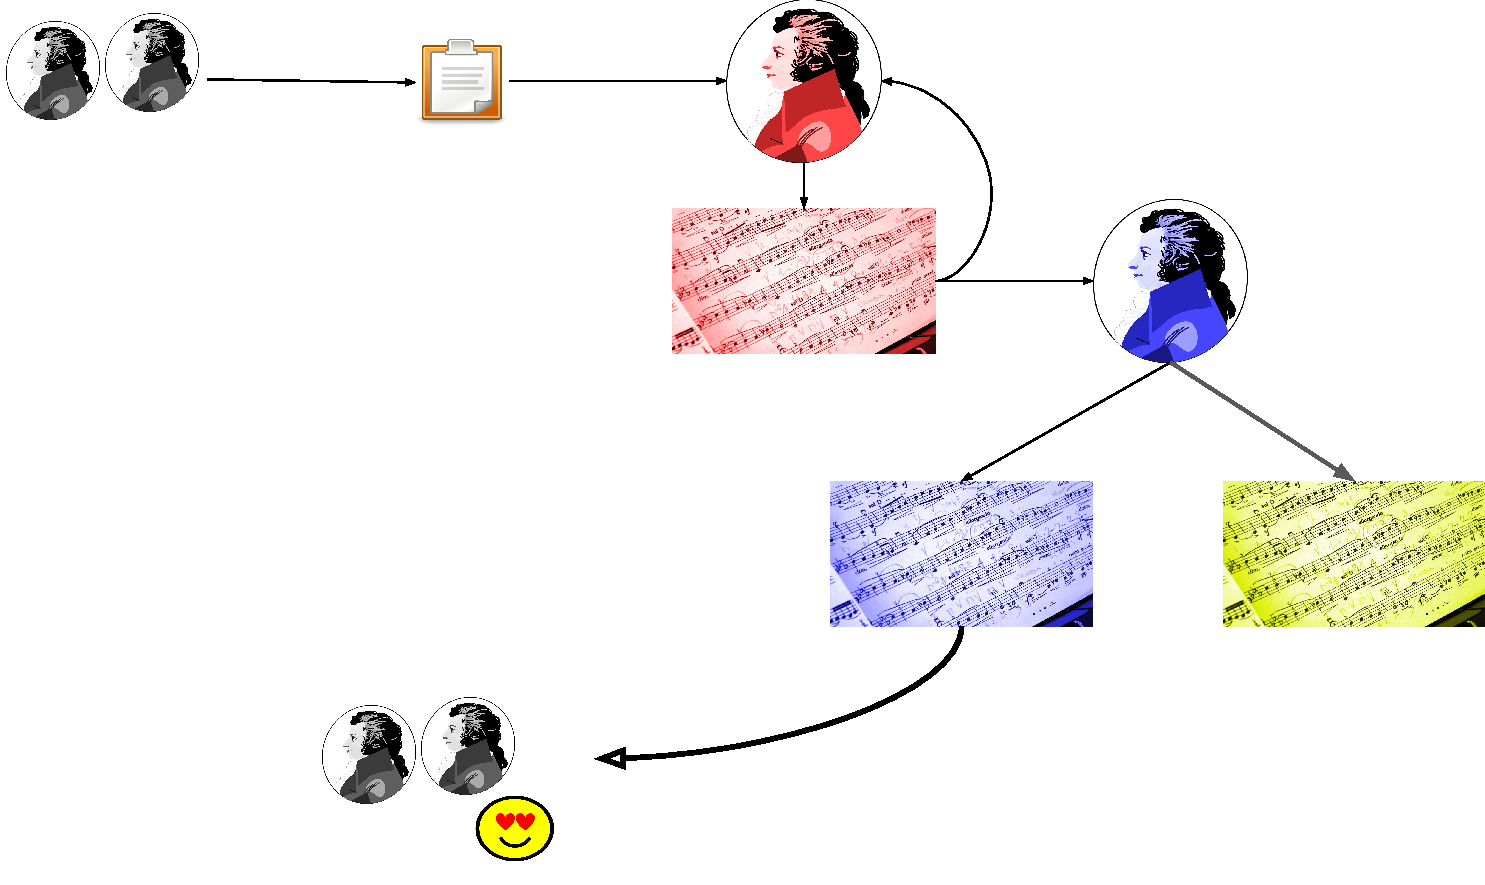
\includegraphics[scale=0.35]{multicomposer.pdf}
	\caption{Use Case 2: Multiple composers define a SharedPlan. Composer 1 (\textcolor{red}{red}) starts
	iterating, commits a work-in-progress and defines a sub-plan. Composer 2 (\textcolor{blue}{blue}) retrieves the sub-plan and continues iterating until the original composers are
	satisified. Composer 2 maintains a separate branch for personal investigation.}
	\label{fig:multicomposer}
\end{figure}

 \todo[inline]{Mark}

Our second use case considers the case where multiple composers create a music specification together, and then collaboratively compose music that stays on track with the original specification.

\subsection{Therapist with Agent - Human Composition Team}

\begin{figure}
	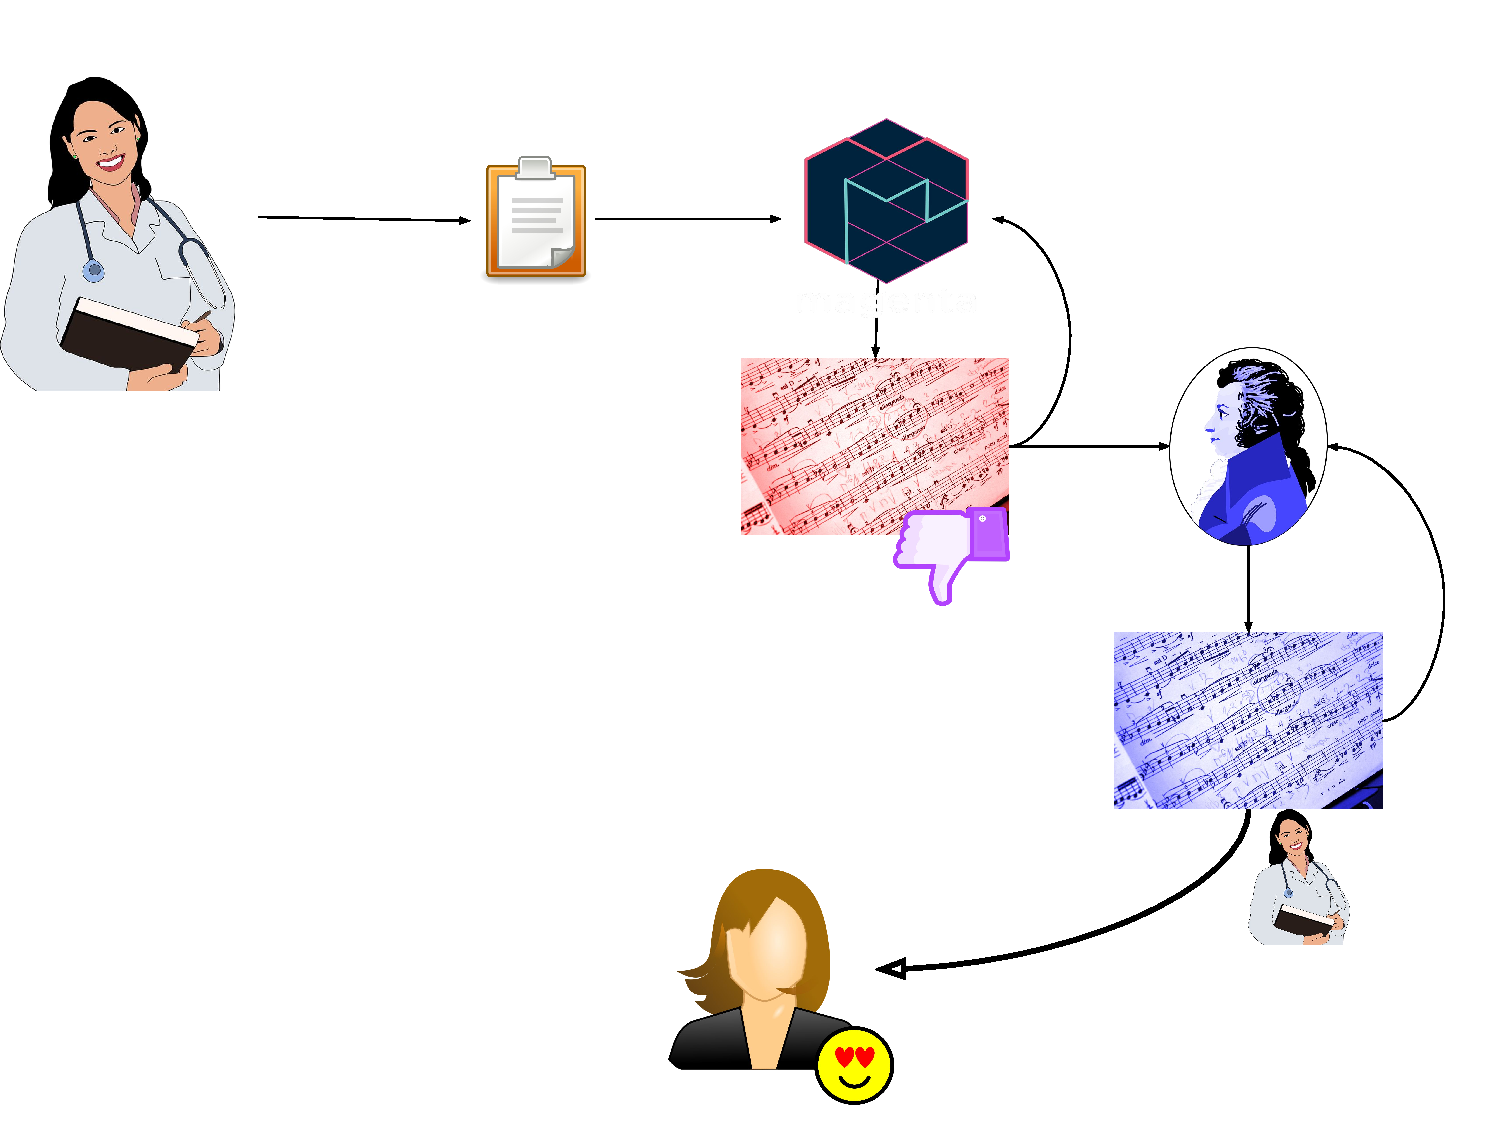
\includegraphics[scale=0.35]{clinical.pdf}
	\caption{Use Case 3: A clinician defines a SharedPlan with more complex metadata for theraputic use. An agent performs the initial composition which consists of the bulk of the work.	A human composer reviews the work and makes minor adjustments. The clinician approves the work and provides the result to the patient for treatment.}
	\label{fig:clinical}
\end{figure}

Our third case considers the situation where a music therapist treats their patients using newly composed music, specific to a given patient's needs. Music therapy is used in many contexts such as the treatment of autism. This SharedPlan may have a more highly-refined specification than music for casual listening, such as a specific tempo or special therapeutic timbres (sound qualities). 

In this case, due to high volume of personal treatment plans, the initial SharedPlan is executed by an agent which performs the bulk of the composition. The agent's composition is then reviewed by a human who may make only small modifications to make the music more warm or less mechanical. The clinician makes the final approval and then provides the music to the patient for treatment.


\section{Evaluation Methodology}

 \todo[inline]{Mark}

% testing this is quite lengthy. It involves people writing a piece! That said, clearly computer scientists must find ways to evaluate success on long term studies. There are plenty of things in life that computers can facilitate, that are not easy or quick to evaluate.

%this will probably be a small study on trained musicians rather than a large-scale crowdsourced study

%import metric to see what percentage of suggestions each user takes. In fact, this measurement has some more significance.... it not only describes the success of the system's suggestions but also the personality of each composer (do they accept suggestions or always do things on their own). I wonder what other kinds of activities could evaluate a composer's personality profile with respect to this quality. That could even be addressed without our system, just with simple collaboration activities. That would not only be interesting and important to learn about the composers, but also important for eventually evaluating the rate of suggestions accepted by the system

% We can test version control / metadata / intention sharing by comparing composers' experiences emailing each other ideas versus using our system.

% To test the usefulness of suggestions, we can compare composers using our revision / metadata system without system analysis and suggestions versus with analysis and suggestions. This could be further broken up by measuring differences between showing analysis percentages but not giving suggestions, versus giving suggestions.

% composers vote on whether or not the piece sounds like it reached the goal.

\section{Discussion}

 \todo[inline]{David + Mark}
\subsection{Enhancing or Stifling Creativity}

Notes: evaluation is optional. Can be ignored by committer.

\subsection{Limitations}

There are several limitations in this proposal that are inherent in the design. This is purposeful as addressing these limitations may result in undo expansion of intent, scope, or problem tractability. Nevertheless, it is important to be explicit about known limitations.

\textit{No explicit improvisation support.} The collaborative design is inspired from software engineering teamwork, which is a solidary activity. Unlike software, in music very fruitful results may occur in real-time improvisation by several musicians. The design does not preclude improvisation but does not account for it either. There may be interesting paths to explore discovered during improvisation that would not be captured by this design. A composer would have to create separate branches and record improvisation sections in each branch. The design does not account for partial interchange between branches.

\textit{Model may not generalize.} While we are confident that SharedPlans, software revision control and algorithmic evaluation is applicable to music composition, it is uncertain that the overall framework can be generalized to other domains. For example, it is difficult to imagine using this design for creating visual artwork. Revision control on binary formats is not very useful. Algorithmic evaluation of intent of a painting appears to be far more difficult than music. Music has a historically long interplay with mathematics making algorithmic evaluation more tractable. 

\textit{Representation is discrete MIDI, not sounds. Vocals are not supported.} MIDI is far easier to generate and maintain under version control. This implies that many interesting sounds such as vocals, ocean waves and many experimental musical forms cannot be expressed in the current design. MusicXML is another text-based format that is more flexible than MIDI while still being amenable to revision control. However, it does not support vocals and more sophisticated sounds either. 

\textit{Corpus based shared beliefs may not be robust.} One of the key assumptions is that genre / mood permutations generate a reasonable representation of the intent of the music. This representation is corpus based. This assumption presumes that genre and mood classification solutions exist, particularly for information retrieval procedures and that the representation is robust enough for the evaluation function to provide useful guidance. Since this has not been built and validated, the certainty of this assumption remains a source of further investigation.


%\todo[inline]{Mark}
%Are there any generalizations of the automated analysis? It's a special case of semantic analysis that is specific to temporal structure. What would it be like to work on a story? The focus should be on considering things that do not rely on external crowdsourced work (point made in IdeaHound).

%\todo[inline]{Mark}
%Current music representation is discrete MIDI, not audio. Limits for vocals, ocean sounds. MIDI not Music XML. Sure, MIDI blocks could be used as placeholders for later-inserted, real-audio sounds, but it would be nice to avoid the need for future post-production work. Would be nice for composers to collaborate and have a finished piece art the end of the collaboration.


\section {Future work}

 \todo[inline]{David + Mark}
 
\begin{itemize}

\item Originality Evaluation, derivative work - do new compositions potentially expose intellectual property infringement.

\item integration with existing DAW, especially for layering notion of blocks over an existing piece.

\item MusicXML
\todo[inline]{Mark: MusicXML instead of MIDI. Makes automatic evaluation more difficult} 

\item Improved agent composition
\todo[inline]{David: 1. maybe re-mention here how could work when human agents communicate their intentions concisely and formally. 2. reinforcement learning} 

\item Intelligent ad hoc composition
\todo[inline]{David: what would this be?} 

\item Facilitator of scalable music composition
\todo[inline]{David: How is this different? What what change? is it the ``scalable" aspect?} 

\item improved evaluator
\todo[inline]{Mark: Improved evaluator. Multiple mutual information for interacting parameters of music.} 

% THESE ARE EXTENSIONS TO HOW WE COULD IMPROVE THE ANALYSIS (DO NOT DELETE)

%In the manifesto, Widner recalls key points made by theorist Cohen in the 1950s, that an information approach for describing music must develop to account for two things crucial to music but not included in information theory (at Cohen's time but still hardly so half a century later) 1) there must be a theory of interactions for multiple streams of musical information, for example for the way in which rhythmic information may make harmonic events more or less certain. Composers do not decide all of music's parameters separately. 2) there must be theory for account for multiple levels of structural hierarchy coming at once from a single stream of musical information. Rhythms constitute a local time feel but also accelerate a piece toward new sections. Recent directions in information theory may provide insight. 

%The first point requires a generalization of mutual information to multiple random variables, which has been difficult to interpret and met with confusion over several coexistent approaches [V.d. Cruys 2011]. Multivariate mutual information is used to describe the extent to which the knowledge of one event can reduce the entropy in several other variables. To our knowledge, the second point has not yet been explored.

%Cohen Quotes
%1. the basic [assumption] is that statistical probability... corresponds to the listener's expectations... the average surprisal value... represents the listener's state of uncertainty?
%2. ?Another... is that one portion of the cultural sign system can be legitimately abstracted from the whole, and that values based on this abstraction will have the same worth as when the portion is a part of the whole.?
%3. ?A further assumption... a sequence of musical events is experienced on only one architectonic level: in melodic analyses, on the level of notes or intervals; in rhythmic analyses, on the level of the pulse pattern... theory will have to take account of the interaction among levels.?
%We need to consider several streams of info. and their interactions: rhythm, pitch, harmony, timbre. Even within one type of information stream, say pitch, we need to consider several hierarchical levels at once: 
\end{itemize}

\section{Conclusion}
  
Our proposal contributes in two novel areas of collaborative music composition:
\begin{itemize}
	\item A workflow incorporating SharedPlans including intentionality and sub-plans, Collaborative Ideation, revision control Intentionality, SharedPlan and Agents
	\item An algorithmic evaluation of the composition against intention, to ensure that both human and agent composers cooperate in reaching the shared objective.
\end{itemize}

As discussed in the Future Work, we see this initial proposal as a start of interesting area to explore leading to improved creativity, diversity and applicability of music composition as a tool for composers, music therapists and listener pleasure.

 \todo[inline]{David + Mark}
 
 \todo[inline]{Mark: Probably important to mention again how this is an extention to things like SoundCloud and Blend}

\section{References}

 \todo[inline]{David + Mark: clean this up, add proper citations in text}
 
IdeaHound: Improving Large-scale Collaborative Ideation with Crowd-powered Real-time Semantic Modeling
P Siangliulue, J Chan, SP Dow, KZ Gajos
Proceedings of the 29th Annual Symposium on User Interface Software and ...
2016

Toward collaborative ideation at scale: Leveraging ideas from others to generate more creative and diverse ideas
P Siangliulue, KC Arnold, KZ Gajos, SP Dow
Proceedings of the 18th ACM Conference on Computer Supported Cooperative ...
2015

ChordRipple Anna Huang, Gajos

Meyer, L.B., 1956. Emotion and Meaning in Music. Chicago University Press, Chicago, IL.

Narmour, E.. 1992. The Analysis and Cognition of Melodic Complexity: The Implication-Realization Model.

D. Huron. 2006. Sweet Anticipation: Music and the Psychology of Expectation. MIT Press, Cambridge, MA.

Abdallah, Cognitive Music Modeling: An Information Dynamics Approach. 2012 3rd International Workshop on Cognitive Information Processing (CIP)

Widmer, Gerhard. 2016. Getting closer to the essence of music: The Con Espressione manifesto. ACM Transactions on Intelligent Systems and Technology

Engel et al., Neural Audio Synthesis of Musical Notes with WaveNet Autoencoders, 2017

Wiggins, Auditory Expectation: The Information Dynamics of Music Perception and Cognition. 2012 Topics in Cognitive Science

Moles, A.. 1966. Information Theory and Aesthetic Perception. University of Illinois Press, Urbana, IL

Two Multivariate generalizations of Pointwise Mutual Information Tim Van de Cruys, Association for Computational Linguistics 2011

Cohen, Joel E., Information Theory and Music , Behavioral Science, 7:2 (1962:Apr.) p.137

Schillinger, Joseph The mathematical basis of the arts 1948

Pierce, Electronics, waves, and messages. 1956

Pierce, Letter Scientific American 1956

Youngblood, Style as information 1958 Journal of Music Theory

The mathematical theory of communication. Shannon, Claude Elwood 1948. Bell Tel Labs Monograph

Torvalds, Linus, and Junio Hamano. "Git: Fast version control system." URL http://git-scm. com (2010).

\todo[inline]{Fix references from section to section}

\bibliographystyle{elsarticle-num-names}
\bibliography{harmonia-bib}

\end{document}

%\subsection{Citations}

% MUST ADD ENTRY TO BIB FILE FIRST

%Here are two examples of how to cite a paper properly:
%\begin{itemize}
%	\item \citet{bernstein2000complexity} shows that ... 
%	\item Prior work has shown that ... \citep{bernstein2000complexity}.
%\end{itemize}

%%  \citet{key}  ==>>  Jones et al. (1990)
%%  \citep{key}  ==>>  (Jones et al., 1990)




%% The Appendices part is started with the command \appendix;
%% appendix sections are then done as normal sections
%% \appendix

%% \section{}
%% \label{}

%% References
%%
%% Following citation commands can be used in the body text:
%%
%%  \citet{key}  ==>>  Jones et al. (1990)
%%  \citep{key}  ==>>  (Jones et al., 1990)
%%
%% Multiple citations as normal:
%% \citep{key1,key2}         ==>> (Jones et al., 1990; Smith, 1989)
%%                            or  (Jones et al., 1990, 1991)
%%                            or  (Jones et al., 1990a,b)
%% \cite{key} is the equivalent of \citet{key} in author-year mode
%%
%% Full author lists may be forced with \citet* or \citep*, e.g.
%%   \citep*{key}            ==>> (Jones, Baker, and Williams, 1990)
%%
%% Optional notes as:
%%   \citep[chap. 2]{key}    ==>> (Jones et al., 1990, chap. 2)
%%   \citep[e.g.,][]{key}    ==>> (e.g., Jones et al., 1990)
%%   \citep[see][pg. 34]{key}==>> (see Jones et al., 1990, pg. 34)
%%  (Note: in standard LaTeX, only one note is allowed, after the ref.
%%   Here, one note is like the standard, two make pre- and post-notes.)
%%
%%   \citealt{key}          ==>> Jones et al. 1990
%%   \citealt*{key}         ==>> Jones, Baker, and Williams 1990
%%   \citealp{key}          ==>> Jones et al., 1990
%%   \citealp*{key}         ==>> Jones, Baker, and Williams, 1990
%%
%% Additional citation possibilities
%%   \citeauthor{key}       ==>> Jones et al.
%%   \citeauthor*{key}      ==>> Jones, Baker, and Williams
%%   \citeyear{key}         ==>> 1990
%%   \citeyearpar{key}      ==>> (1990)
%%   \citetext{priv. comm.} ==>> (priv. comm.)
%%   \citenum{key}          ==>> 11 [non-superscripted]
%% Note: full author lists depends on whether the bib style supports them;
%%       if not, the abbreviated list is printed even when full requested.
%%
%% For names like della Robbia at the start of a sentence, use
%%   \Citet{dRob98}         ==>> Della Robbia (1998)
%%   \Citep{dRob98}         ==>> (Della Robbia, 1998)
%%   \Citeauthor{dRob98}    ==>> Della Robbia


%% References with bibTeX database:

